\subsection{Hyperball-line picking}
\label{sec:hyperball_line}

The (closed) $n$-Dimensional hyperball (or just s$n$-ball) is the set
of points $B^n = \big\{ {\mathbf x} \in \R^n \; \big| \; \|{\mathbf x} \|_2 \leq R
\big\},$ where $R$ is the {\em radius}. For instance:
\begin{itemize}

\item A 1-ball is a line segment;

\item A 2-ball is a disk;

\item A 3-ball is an ordinary ball, i.e., the interior of a sphere.

\end{itemize}
In general, an $n$-ball is the interior of a $n-1$-sphere. 
% http://en.wikipedia.org/wiki/N-sphere

Figure~\ref{fig:hyperball_eg} shows an example of the line-picking
problem on the 2-ball (the disk). Generating points uniformly in an
$n-ball$ can be done by rejection (e.g., generating points uniformly
on an enclosing $n$-cube and sampling only those in the ball), or by
\begin{enumerate}

\item Choosing points uniformly on the surface. This can be
  accomplished by taking
  \begin{equation}
    \label{eq:x_surface_sphere}
    \x = R \frac{\y}{\| \y \|_2}, 
  \end{equation}
  where the $y_i \sim N(0,1)$ are IID standard normal random variates.

\item The find a point inside the $n$-ball by taking $u^{1/n} \x$,
  where $u \sim U([0,1])$ is uniformly generated from the interval $[0,1]$.

\end{enumerate}
The result is a set of points chosen so that the probability of there
being $k$ points inside non-overlapping regions of volume $v$ takes
IID Poisson distributions with mean $\lambda v$ where $\lambda =
m/V_n$, where $m$ is the total number of points generated, and $V_n$
is the volume of the $n$-ball.


\begin{figure}[tbp]
  \begin{center}
    \subfloat[\label{fig:hyperball_eg}2-ball
    example.]{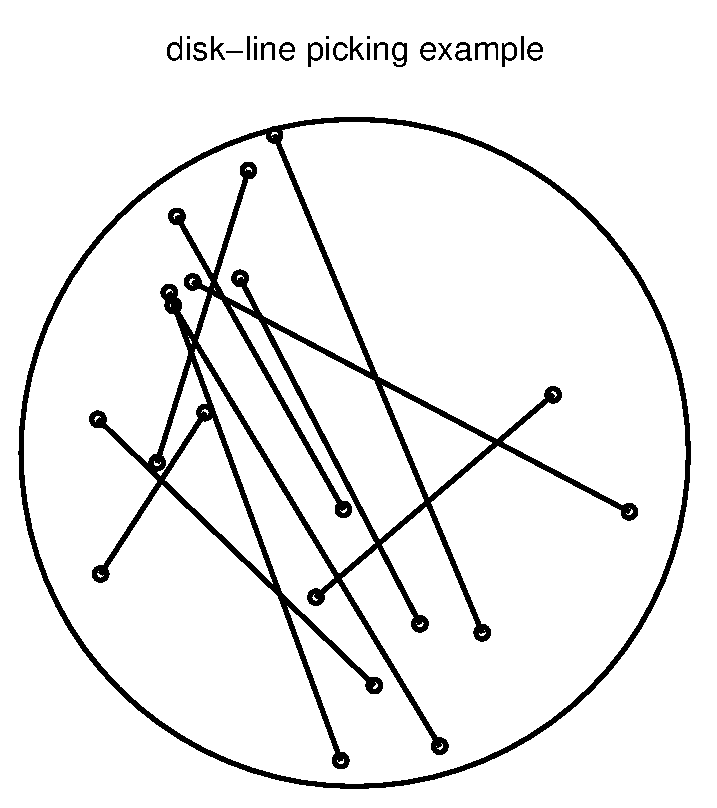
\includegraphics[width=0.4\columnwidth]{../Matlab/Plots/LinePicking_test_sim_disk_eg.eps}} 
    \hspace{6mm}
    \subfloat[\label{fig:hyperball_pdf}PDF of $n$-balls.]{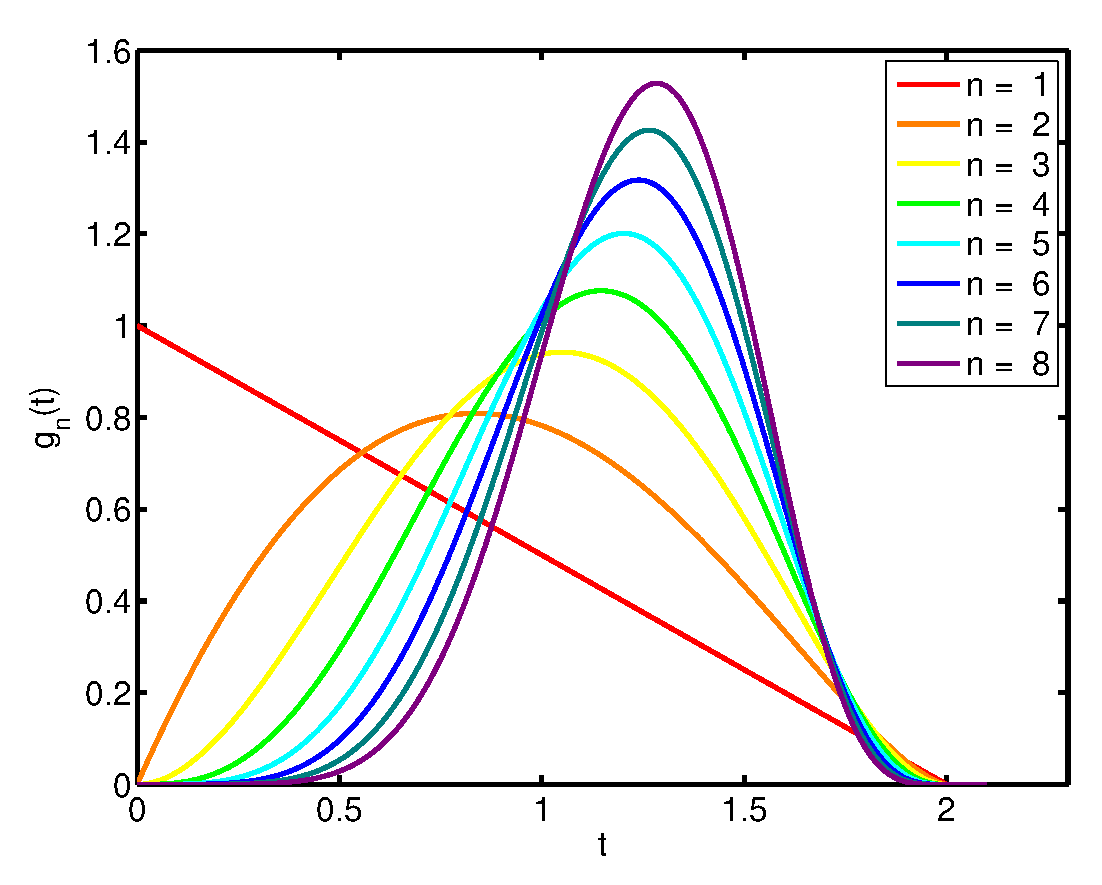
\includegraphics[width=0.48\columnwidth]{../Matlab/Plots/LinePicking_test_balls.eps}}
    \caption{The hyperball-line picking problem.}
  \end{center} 
\vspace{-4mm}
\end{figure}

\subsubsection{PDF}

Another obvious region on which to solve the line-picking problem is
the ball in $n$-dimensions~\cite{tu00:_circle_line} (equations
(27-31)). For a $n$-dimensional ball of radius $R$,
\begin{equation}
 g^{n-{\rm ball}}_R(t) = n \frac{t^{n-1}}{R^n} I_x\left( 
  \frac{1}{2} (n+1), \frac{1}{2}
                      \right),
\end{equation}
where
\begin{equation}
 x = 1 - \frac{t^2}{4 R^2}, 
\end{equation}
and $I_x(p,q)$ is a {\em regularized beta function}
\begin{equation}
   I_x(p,q) = \frac{ B(x; p,q)}{B(p,q)},
\end{equation}
where $B(x; p,q)$ is an incomplete beta function, and $B(p,q)$ is a
beta function, i.e., 
\begin{eqnarray}
  B(p,q)    & = & \int_0^1 t^{p-1} (1 - t)^{q-1} \, dt =
  \frac{\Gamma(p) \Gamma(q)}{\Gamma(p+q)}, \\
  B(x; p,q) & = & \int_0^x t^{p-1} (1 - t)^{q-1} \, dt.
\end{eqnarray}
The first few of these are \cite{tu00:_circle_line} ($P_2$ in (5) and
(17), $P_3$ in (9) and (19), $P_4$ in (18) and $P_5$ in (20), general
even form in (15), general odd form in (16)):
\begin{eqnarray}
  \label{eq:ball_line_picking}
  g^{1-{\rm ball}}_R(t) & = & \frac{1}{R} - \frac{t}{2 R}   \label{eq:line_line_picking}, \\
  g^{2-{\rm ball}}_R(t) & = & \frac{4 t}{\pi R^2} \cos^{-1} \left( \frac{t}{2R} \right)
               - \frac{2 t^2}{\pi R^3} \sqrt{1 - \frac{t^2}{4 R^2} } \label{eq:2dball_line_picking} , \\
          & = & \frac{2 t}{R^2} 
               - \frac{2 t^2}{\pi R^3} \sqrt{1 - \frac{t^2}{4 R^2} }
               - \frac{4 t}{\pi R^2} \sin^{-1} \left( \frac{t}{2R} \right) \label{eq:2dball_line_picking2} ,  \\
  g^{3-{\rm ball}}_R(t) & = & \frac{3 t^2}{R^3} - \frac{9 t^3}{4 R^4} + \frac{3 t^5}{16 R^6}   \label{eq:sphere_line_picking}  , \\
  g^{4-{\rm ball}}_R(t) & = &  \frac{8 t^3}{\pi R^4} \cos^{-1} \left( \frac{t}{2R} \right) 
              - \frac{8 t^4}{3 \pi R^5} \left( 1 - \frac{t^2}{4 R^2} \right)^{3/2}
               - \frac{4 t^4}{\pi R^5} \sqrt{1 - \frac{t^2}{4 R^2} } \\
  g^{5-{\rm ball}}_R(t) & = & \frac{5 t^4}{R^5} - \frac{75 t^6}{16 R^6} + \frac{25 t^7}{32 R^8} - \frac{15 t^9}{256 R^{10}} .
  \label{eq:ball_line_picking-end}
\end{eqnarray}
Tu and Fischbach \cite{tu00:_circle_line} also extend these results to
cases with non-uniform point distributions.
 
Figure~\ref{fig:hyperball_pdf} shows a comparison of line picking on
balls of various dimensions, and Figure~\ref{fig:various} shows a
comparison of the 2D and 3D balls to the square and cube. We can see
that as long as the areas (volumes) are matched, they appear quite
similar, respectively, though the rectangle varies considerably more.
% plot is similar to http://mathworld.wolfram.com/BallLinePicking.html

\subsubsection{CDF}

Take the case $R=1/2$ (we extend to the general case below), so that
\begin{equation}
 g^{n-{\rm ball}}_{1/2}(t) = n 2^n t^{n-1} I_{1-t^2}\left( 
  \frac{1}{2} (n+1), \frac{1}{2}
                      \right),
\end{equation}
where
\begin{equation}
   I_{1-t^2}(p,q) = 1 - I_{t^2}(q,p) = 1 - \frac{ B(t^2; q,p)}{B(q,p)}.
\end{equation}
So the CDF
\begin{eqnarray}
   G^{n-{\rm ball}}_{1/2}(\tau)
       & = & \int_0^\tau g^{n-{\rm ball}}_{1/2}(t) \, dt \nonumber \\
       & = &  \int_0^\tau n 2^n t^{n-1} \, dt 
            - \int_0^\tau n 2^n t^{n-1}  \frac{ B(t^2; q,p)}{B(q,p)} \, dt 
                  \nonumber \\
       & = &  2^n \tau^{n} 
            - \frac{n 2^n}{B(q,p)} \int_0^\tau t^{n-1}   B(t^2; q,p) \, dt .
\end{eqnarray}
Concentrating on the second term, and inserting the definition of the
incomplete $\beta$-function, we get 
\begin{eqnarray}
  n \int_0^\tau t^{n-1}  B(t^2; q,p) \, dt
       & = & n \int_{t=0}^\tau t^{n-1}  \int_{s=0}^{t^2} s^{q-1} (1 - s)^{p-1} \, ds \, dt \nonumber \\
       & = & n \int_{t=0}^\tau \int_{s=0}^{t^2} t^{n-1}  s^{q-1} (1 - s)^{p-1} \, ds \, dt \nonumber \\
       & = & n \int_{s=0}^{\tau^2} \int_{t=\sqrt{s}}^\tau t^{n-1}  s^{q-1} (1 - s)^{p-1} \, dt  \, ds \nonumber \\
       & = & n \int_{s=0}^{\tau^2}  s^{q-1} (1 - s)^{p-1} \int_{t=\sqrt{s}}^\tau t^{n-1} \, dt  \, ds \nonumber \\
       & = & \int_{s=0}^{\tau^2}  s^{q-1} (1 - s)^{p-1} \left[ t^{n} \right]_{t=\sqrt{s}}^\tau  \, ds \nonumber \\
       & = & \tau^n \int_{s=0}^{\tau^2}  s^{q-1} (1 - s)^{p-1} \, ds -
              \int_{s=0}^{\tau^2}  s^{n/2+q-1} (1 - s)^{p-1} \, ds \nonumber \\
       & = & \tau^n B(\tau^2; q,p) -  B(\tau^2; q+n/2,p).
\end{eqnarray}
Substituting back we get
\begin{eqnarray}
   G^{n-{\rm ball}}_{1/2}(\tau)
       & = &  2^n \tau^{n} 
            - \frac{n 2^n}{B(q,p)} \int_0^\tau t^{n-1}   B(t^2; q,p) \, dt  \nonumber \\
       & = &  2^n \left[ \tau^{n} \left(1-   \frac{B(\tau^2; q,p)}{B(q,p)} \right)
                           + \frac{B(\tau^2; q+n/2,p)}{B(q,p)} \right] \nonumber \\
       & = &  2^n \left[ \tau^{n} I_{1-\tau^2}(p,q)  + \frac{B(\tau^2; q+n/2,p)}{B(q,p)} \right],
\end{eqnarray}
where remember $p = \frac{1}{2} (n+1)$, and $q=\frac{1}{2}$.

Extending this to the general case with radius $R$ we get:
\begin{equation}
  \label{eq:cdf_n-ball}  
   G^{n-{\rm ball}}_{R}(\tau)
     =  2^n \left[ \left( \frac{\tau}{2R} \right)^{n} I_{x}(p,q)  + \frac{B(1-x; q+n/2,p)}{B(q,p)} \right].
\end{equation}

\subsubsection{Moments}

The means for the $n$-dimensional ball (with radius 1) are given in
\cite{weisstein:_ball_line_picking} as
\begin{eqnarray}
  \label{eq:ball-ndim-mean}
  \mu^{1D-{\rm ball}} & = & \frac{2}{3}, \\
  \mu^{2D-{\rm ball}} & = & \frac{128}{45 \pi},\\
  \mu^{3D-{\rm ball}} & = & \frac{36}{35}, \\
  \mu^{4D-{\rm ball}} & = & \frac{16384}{4725 \pi}.
\end{eqnarray}
The more general form for higher order moments is given in
\cite{tu00:_circle_line}~(138-141) as
\begin{eqnarray}
  \label{eq:ball-ndim-moments}
  \alpha_m^{n-{\rm ball}} & = &
     \frac{n 2^{m+n}}{m+n} \frac{B\left(\frac{n+1}{2}, \frac{n+m+1}{2}  \right)}{B\left(\frac{n+1}{2}, \frac{1}{2} \right)} R^m, \\
       & = & \left( \frac{n}{n+m} \right)^2 
                 \frac{\Gamma\left( n+m+1 \right) \Gamma\left( n/2 \right) }
                      {\Gamma\left( (n+m)/2 \right) \Gamma\left( n+1 + m/2 \right) } R^m.  
\end{eqnarray}
Obviously, central moments can be derived in the standard way.





